\documentclass{standalone}
\newcommand{\FontPath}{../../../assets/fonts/} 
\usepackage{fontspec}
\usepackage{unicode-math}

% Thiết lập phông chữ
\setmainfont{STIX Two Text}
\setsansfont{STIX Two Text}
\setmonofont{STIX Two Text}
\setmathfont{STIX Two Math}


\usepackage{xcolor}
\definecolor{quartoText}{RGB}{33, 37, 41} % Màu văn bản chính từ theme default của quarto
    
\usepackage{tikz}
\usetikzlibrary{arrows, positioning, calc}

% Đảm bảo mọi nội dung trong tikzpicture đều dùng màu văn bản chính
\AtBeginEnvironment{tikzpicture}{\color{quartoText}}
\begin{document}
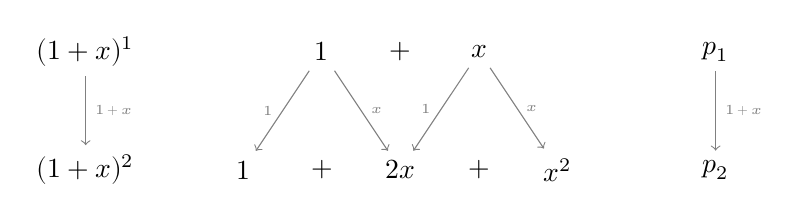
\begin{tikzpicture}
    % Dòng thứ nhất
    \node (d11) at (-1,12) {$1$};
    \node (d12) at (0,12) {$+$};
    \node (d13) at (1,12) {$x$};
    
    % Dòng thứ hai
    \node (d21) at (-2, 10.5) {$1$};
    \node (d22) at (-1, 10.5) {$+$};
    \node (d23) at (0, 10.5) {$2x$};
    \node (d24) at (1, 10.5) {$+$};
    \node (d25) at (2, 10.5) {$x^2$};

    % Các nhị thức tương ứng
    \node (d1l) at (-4,12) {$(1+x)^1$};
    \node (d2l) at (-4,10.5) {$(1+x)^2$};
    \node (d1r) at (4,12) {$p_1$};
    \node (d2r) at (4,10.5) {$p_2$};
    
    % Các đoạn thẳng
    \begin{scope}[every path/.style={color=gray}, every node/.style={color=gray,font=\tiny}]  
    \draw [->] (d11)--(d21) node[midway, left] {$1$};
    \draw [->] (d11)--(d23) node[midway, right] {$x$};
    \draw [->] (d13)--(d23) node[midway, left] {$1$};
    \draw [->] (d13)--(d25) node[midway, right] {$x$};

    \draw [->] (d1l)--(d2l) node[midway,right] {$1+x$};
    \draw [->] (d1r)--(d2r) node[midway,right] {$1+x$};
    \end{scope}
\end{tikzpicture}
\end{document}